\documentclass[UTF8]{ctexrep}

\usepackage{fontspec}
\usepackage{graphicx}

%--------------------------%

\setmonofont{Consolas}
\ctexset{
    section/name = {第,节},
    section/number = {\arabic{section}},
    subsection/number = {\arabic{section}.\arabic{subsection}}
}

\title{郑和后台计划}

\bibliographystyle{acm}

\begin{document}
\maketitle
\newpage


%--------------------------%
\begin{figure}[h]
    \caption{整体架构}
    \centering
    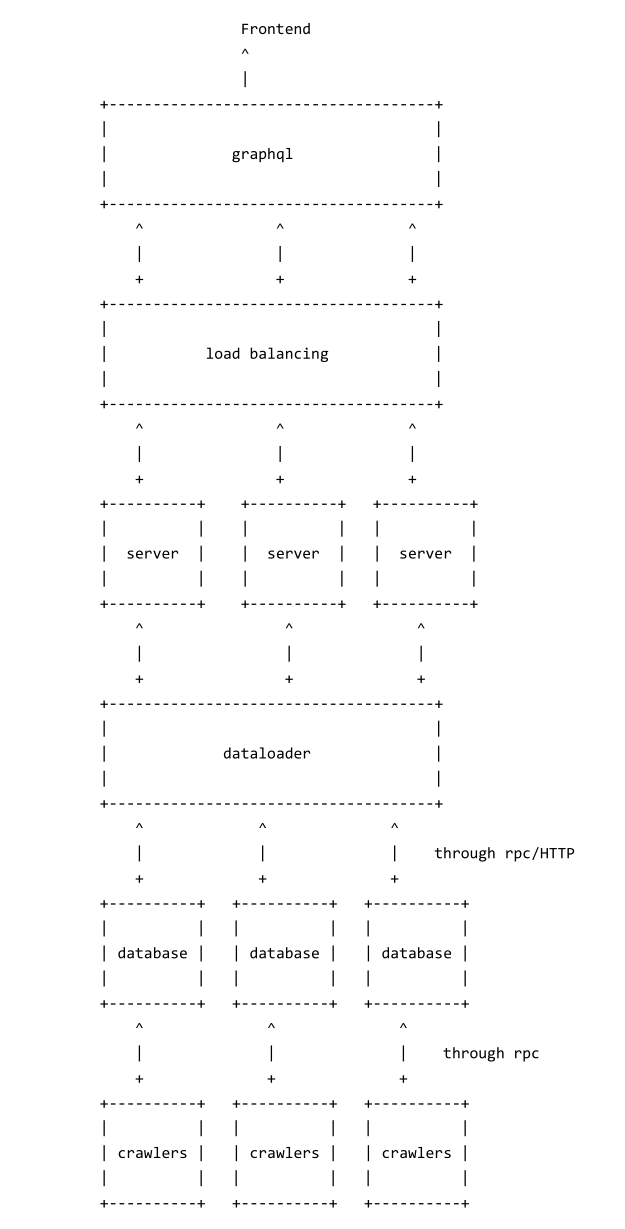
\includegraphics[width=0.75\textwidth]{assets/figures/arch2.png}
    \label{fig:arch}
\end{figure}
\part{数据获取}

%--------------------------%

\part{数据存储}

\section{与爬虫对接}

\paragraph{需求分析}

需要约定接口,对获取到的数据类型及内容进行约束。

\paragraph{Protocal Buffer}

是著名科技公司\textmd{Google}提出的与语言无关,与平台无关,可扩展的用于序列化结构化数据的机制,类似\texttt{XML}和\texttt{JSON}但更简单也更快速。

\par
通过定义\texttt{.proto}的接口文件,规定好需要存储的数据的类型、结构、大小等,更方便进行存储。

\paragraph{RPC}

同样通过\texttt{Protobuf}定义\texttt{RPC Service}需要的参数与格式,供爬虫方调用。

\paragraph{可能存在的问题}

\begin{itemize}
    \item 爬虫获取到不在定义中的数据
    \item 新的数据与已有数据重复或冲突
    \item 存储失败后如何重新存储
\end{itemize}

\section{数据库的选择}

\paragraph{需求分析}

存储需要做到:
\begin{itemize}
    \item 体现数据之间的关联
    \item 可扩展性高
    \item 可存储的数据量大
    \item 根据数据间的联系快速搜索
\end{itemize}

因此我们选用了图数据库\texttt{Dgraph}\footnote{https://dgraph.io}作为存储数据库。

\paragraph{特点}

\texttt{Dgraph}具有以下特点:

\begin{itemize}
    \item 分布式——可以部署在多台服务器上,减轻服务器压力
    \item 快速——能快速对查询进行相应
    \item 高可用性——自动进行同步复制,重启失败的实例
    \item 事务支持——保证数据的一致性
    \item 灵活——随时可调整数据的模式
\end{itemize}

\paragraph{存在的问题}

首先,查询语句不够成熟。
\par
采用了一套自定义的查询语句,不易维护,且语法较为晦涩
\par
其次,该项目比较年轻,不稳定。

\paragraph{主库与从库}

由于需要对获取来的数据进行整合、聚类、分析等准备工作,因此设置\emph{主库与从库},主库中为已经经过处理过的数据,主要用来给用户展示等。而爬虫获取到的数据则直接写入从库,经过处理后再统一与主库进行合并。

\par

采用主库与从库分离的方式,一方面方便对数据的分析与整理;另一方面由主库主要负责读操作、从库主要负责写操作,减轻同时读写对数据库带来的压力。

\paragraph{可能存在的问题}

\begin{itemize}
    \item 如何正确地合并两个库
    \item 如何保证数据一致性、不丢失
    \item 如何从从库中获取数据并异步处理
\end{itemize}

%--------------------------%

\part{数据搜索}

%--------------------------%

\end{document}
